 \chapter{Background} \label{bg}
 \section{Supervised and Unsupervised learning}
 While the models and applications of machine learning are numerous and cover many varied domains and problems, at a fundamental level, machine learning addresses three classes of problems: the problem of uncovering a mapping from an input to an output, learning how policies through experience, and the problem of uncovering interesting and meaningful structure and patterns in a dataset. The first class of problems are commonly referred to as that of Supervised Learning, the second as Reinforcement Learning, and the latter as Unsupervised Learning. For the rest of this thesis, we will mainly concern ourselves with the areas of Supervised and Unsupervised Learning.\\

 In the Supervised Learning setting, models are trained to uncover a mapping $y=f(x)$ between inputs $\mathbf{x}$ and outputs $\mathbf{y}$ in a dataset $\{\mathbf{x}_i, \mathbf{y}_i\} | i=1.. \mathcal{D}$. The source of inputs vary widely, ranging from images to medical information to natural language, with the outputs following a similar pattern. To encode these different sources of inputs and outputs, the inputs and outputs take on mainly two different types: real-valued vectors or nominal/categorical vectors, i.e. $\mathbf{x} \in \mathcal{R}^N$ or $\mathbf{x} \in \{0,1\}^N$ with the same holding for y. For the cases where $y \in \mathcal{R}$, the supervised learning model learns to predict continuous valued outputs, and the task is termed \textit{regression}. The other case, where $\mathbf{y} \in \{0,1\}^N$ the model is trained to predict categorical/binary outputs and the problem is termed \textit{classification}. In the classification task, the model is trained to classify an input $\mathbf{x}$ into one of $N$ possible classes, for example, given medical information about a patient, classify whether the patient has the flu or not. In the regression instance the model is trained to predict a continuous value given the input $x$, for example, given information about a house and its surrounding area predict the price of the house.\\

 In the Unsupervised Learning setting, models are trained to discover interesting patterns inherent in the data. The dataset $\mathbf{x}_i | i=1..\mathcal{D}$ has no label to be classified into or forecasted, and these types of problems tend to be more complicated since they are less well defined \citep{murphy2012machine}. Examples applications of Unsupervised Learning include clustering, topic modelling, generative models, etc.

 \begin{figure}
     \centering
     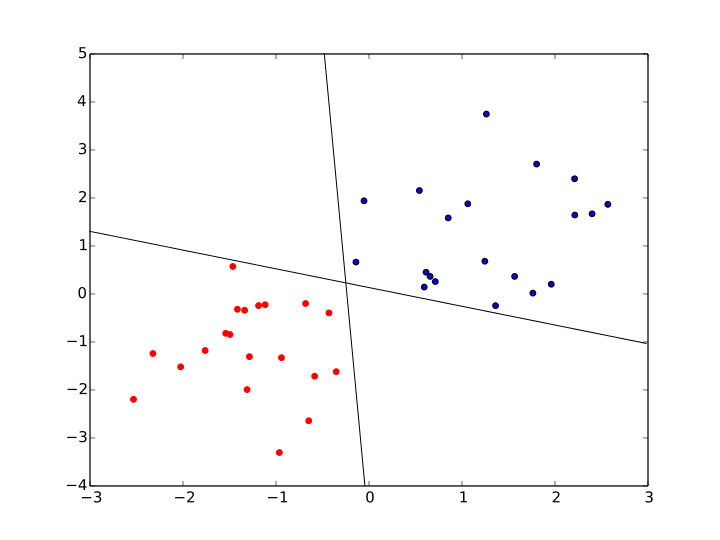
\includegraphics[width=.5\textwidth]{images/KnnClassification}
     \caption{(a) Classification Problem}
     \label{fig:classification}
\end{figure}%

\begin{figure}
     \centering
     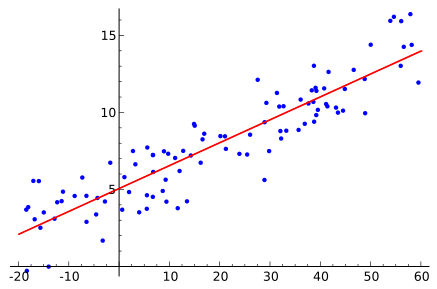
\includegraphics[width=0.5\textwidth]{images/Linear_regression}
     \caption{(b) Regression Problem, \cite{reg}}
     \label{fig:regression}
 \end{figure}


 \citep{murphy2012machine}
 \section{Neural Networks}
 Central to many of the recent advances in machine and deep learning is the perceptron. The perceptron serves as the building block of neural networks and all the consequent derivatives such as convolutional and recurrent neural networks. The perceptron takes a vector of real-valued or ordinal inputs $\mathbf{x_i}$, multiplies each by a weight $\mathbf{W_i}$, applies an activation function $\phi$ to generate an output $y_i$. Formulated mathematically, the perceptron behaves as follows:

 \begin{equation}
     y_i = \phi ( \sum_{j=1}^n w_{ij} x_i) 
 \end{equation}

 where $\phi$ represents the activation function which could be a linear or, more commonly, a non-linear function such as the logistic sigmoid, $\frac{1}{1+e^{-x}}$, the hyperbolic tangent, $\frac{e^{2x} -1}{e^{2x} + 1}$, or the more recently popular rectified linear units \citep{nair2010rectified} $f(x) = max(0,x)$ and exponential linear units \citep{clevert2015fast}, $f(x) = x * (x > 0) + (x < 0) * (\alpha * (e^x - 1))$. The choice of these activation functions is often problem dependent, and has a substantial effect on accuracy and training time. Usually, these activation functions are also increasing, continuous, bounded and differentiable.

 When many of these neurons are stacked we have a layer of neurons, more commonly known as an Artificial Neural Network. Information in the ANN moves forward, from the inputs through the layer of neurons, known as the hidden layer, to the output. By including more neurons in the hidden layer and utilising non-linear activations, the ANN becomes a powerful function approximator that can be efficiently trained to recover functions that map inputs to outputs \cite{murphy2012machine}. ANNs with many hidden layers between the input and output are known as deep neural networks and they are responsible for many state-of-the-art results across the three main areas of machine learning.

 \section{Recurrent neural networks}
 Recurrent neural networks are, at the most fundamental level, neural networks with loops. These loops allow information to persist through time by repeatedly including previous information, stored in a hidden state, in the computations at each time-step. At each time-step, the RNN computes a hidden state h, which can be used to make a prediction on the next element in the sequence. In applications with discrete observations such as language modelling, the prediction at each time-step would be a distribution over a set of possible outcomes, in this case words or characters, given the previous elements in the sequence. Alternatively, RNNs can be trained to predict a single real valued number, or multiple values in a multi-variate time-series forecasting problem such as ours. More rigorously, the RNN models time-series data and makes predictions via the following equations:

 \begin{equation}
     h_n = f(x_n, h_n-1) = g_1(\mathbf{V}_xx_n + \mathbf{V}_hh_{n-1} + \mathbf{c})
 \end{equation}

 \begin{equation}
     y_{out} = f(h_n) = g_2(\mathbf{W}h_n + \mathbf{b})
 \end{equation}

 Where $g_1$ is the activation function applied to every element in the hidden state, and $g_2$ is the activation function applied at the output. The activation at the output could be a softmax for prediction a distribution across a discrete set of outputs, or for continuous regression the logistic sigmoid, the hyperbolic tangent, the popular ReLu \citep{nair2010rectified}, their recent variants the eLu \citep{clevert2015fast} that have been shown to speed up training, or nothing at all. \\

 \begin{figure}
     \centering
     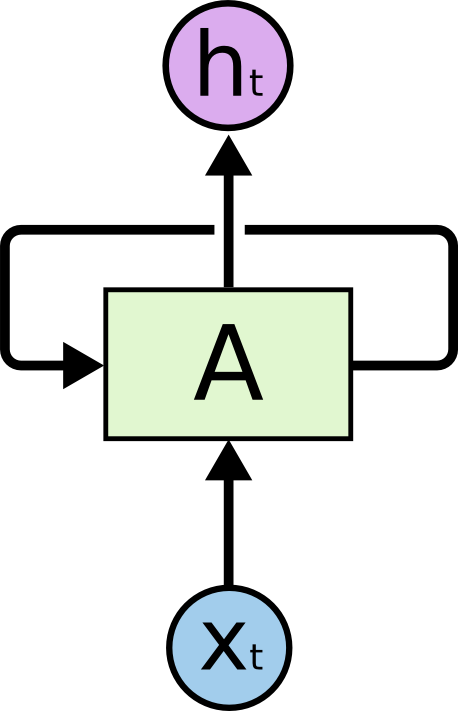
\includegraphics[width=0.2\textwidth]{images/RNN-rolled.png}
     \caption{Rolled RNN, image from http://colah.github.io/posts/2015-08-Understanding-LSTMs/}
     \label{rolled_rnn}
 \end{figure}

 While theoretically RNNs are able to capture information infinitely far in the past, in practice RNNs are 'unrolled' for a finite number of timesteps into the past, over which they are allowed to learn the temporal dependencies. 

 \begin{figure}
     \centering
     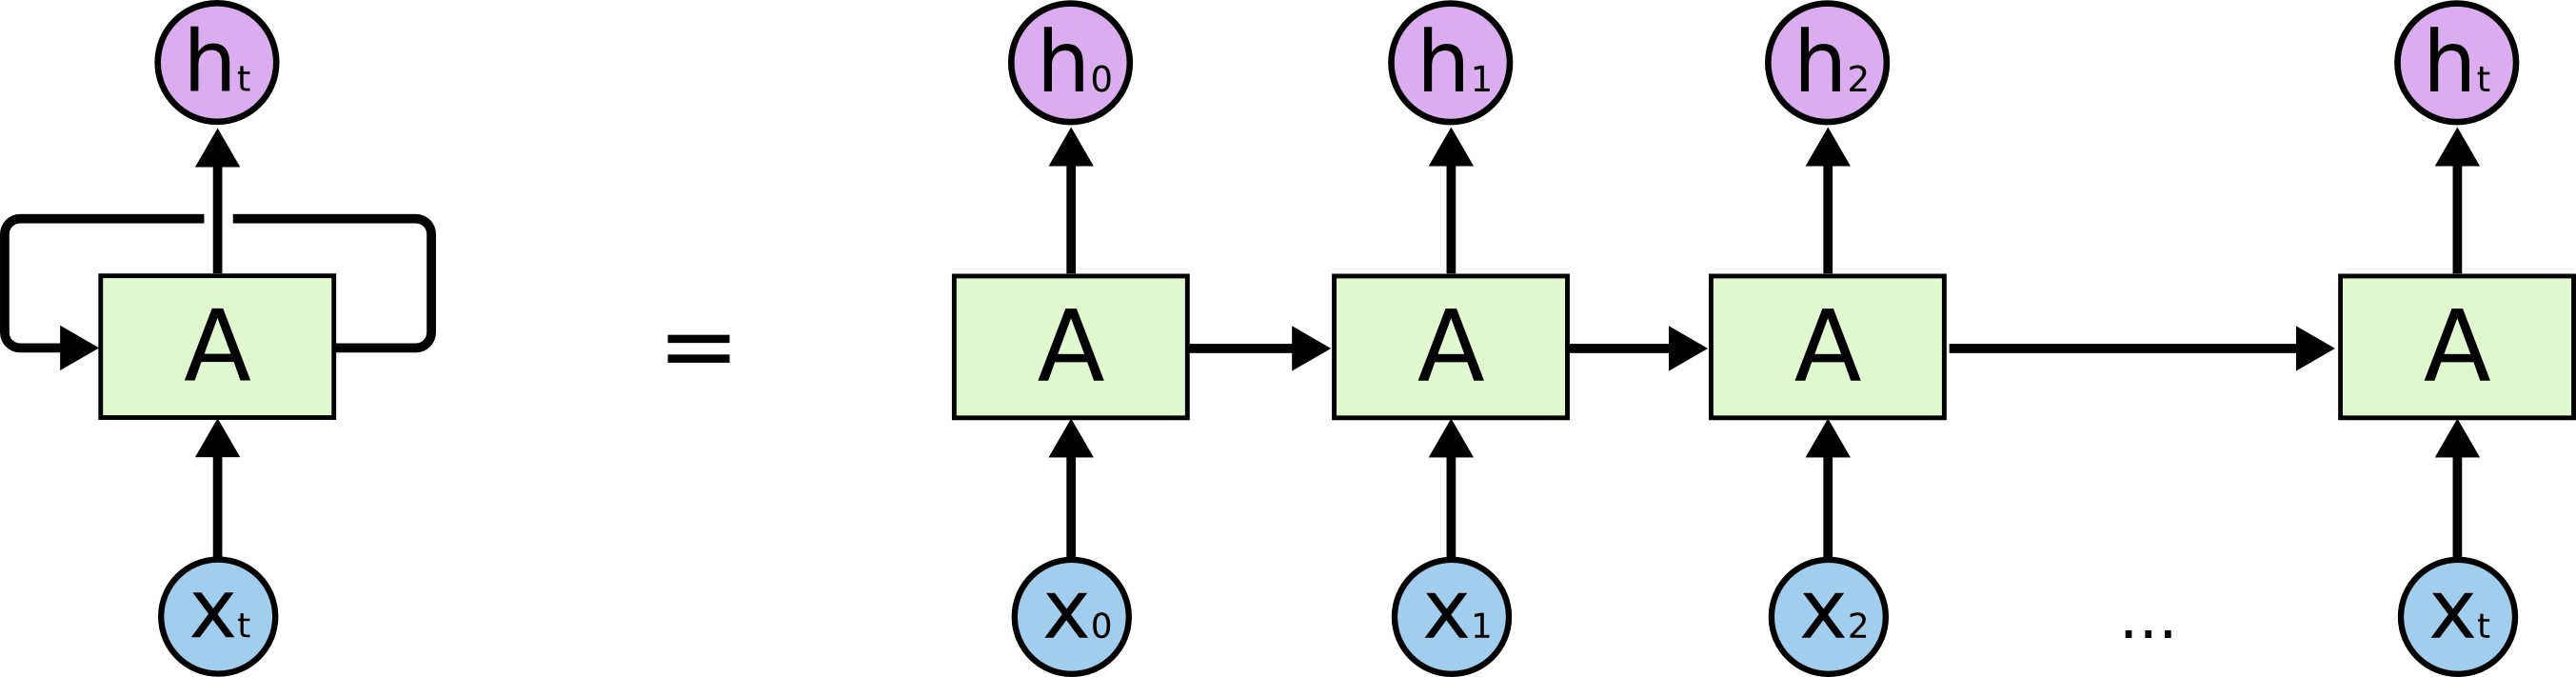
\includegraphics[width=1\textwidth]{images/RNN-unrolled.png}
     \caption{Unrolled RNN, image from http://colah.github.io/posts/2015-08-Understanding-LSTMs/}
     \label{unrolled_rnn}
 \end{figure}

 When unrolled over time and trained to capture dependencies that span over long-ranges, RNNs begin facing the problem of vanishing gradients where the propagation of gradients backwards through time may result in consecutively multiplying many gradients smaller than 1 with each other, such that eventually the gradient approaches 0.\\

 To remedy this, the LSTM \citep{Hochreiter1997} and GRU \citep{Cho2014} have been proposed. These cells overcome the vanishing gradient by introducing two properties, gating and memory. Through gating, these cells are able to propagate gradients backwards essentially through addition thereby circumventing the consecutive multiplication of gradients. Memory cells on the other hand improve the ability to learn long-term dependencies by allowing the LSTM cells to store information in these memory cells, using and overwriting them when needed. In what follows we use an LSTM that implements input, output and forget gates to build its memory cell. These gates respectively allow information into the cell, out of the cell, and cause the LSTM to forget what is stored in memory. Once again, $\mathbf{h}_n$ represents the hidden state of the LSTM cell.

 \begin{equation}
     \begin{split}
         & \mathbf{i}_n  = \sigma(\mathbf{W}_i [\mathbf{x}_{n-1}; \mathbf{h}_{n-1}; \mathbf{c}_{n-1}] + \mathbf{b}_i) \\
         & \mathbf{f}_n  = \sigma(\mathbf{W}_f [\mathbf{x}_{n-1}; \mathbf{h}_{n-1}; \mathbf{c}_{n-1}] + \mathbf{b}_f) \\
         & \mathbf{o}_n  = \sigma(\mathbf{W}_o [\mathbf{x}_{n-1}; \mathbf{h}_{n-1}; \mathbf{c}_{n-1}] + \mathbf{b}_o) \\
         & \mathbf{c}_n =  \mathbf{f}_n \odot \mathbf{c}_{n-1} +  \mathbf{i}_n \odot \mathrm{tanh}(\mathbf{W}_c [\mathbf{x}_{n-1}; \mathbf{h}_{n-1}; \mathbf{c}_{n-1}] + \mathbf{b}_c) \\
         & \mathbf{h}_n =  \mathbf{o}_n \odot \mathrm{tanh}(\mathbf{c}_n)
     \end{split}
 \end{equation}

 \section{Convolutional Neural Networks}
 Convolutional Neural Networks are variants of Vanilla Neural Networks that address the problem of training deep fully connected networks. Convolutional Neural Networks reduce the number of parameters to be learned in a densely connected network by imposing restrictions on the number of neurons in a previous layer any neuron can be connected to \citep{gamboa2017deep}. Groups of neurons, called convolutional filters, share the same weights and process different portions of the input. These filters are convolved with portions of the input, in either 1 or 2 dimensions. The convolutional filters can be convolved with the input to the CNN along any number of dimensions to extract features along those dimensions. For example, a 2D convolutional filter will be convolved with an input image to extract features along both dimensions of an image whereas in the case of input data such as time-series, a 1D convolutional filter can be used and convolved along one dimension, time, to extract temporally relevant features.